% !TEX root = ./report.tex

\clearpage
\section{Background}
\label{background}

\subsection{The Regionalized Value-State Dependence Graph}
\label{background:RVSDG}

The \textit{Regionalized Value-State Dependence Graph}~\cite{RVSDG:HiPEACpaper}
(RVSDG) is a \textit{Directed Acyclic Demand-Based Dependence Graph} (DADBDG),
consisting of nodes representing computations and edges representing the
dependencies between nodes. Each node has inputs and outputs connected through
edges. The arity and order of inputs and outputs depend on the operation the
node represents, as exemplified with the two subsections of node representing
the if-statement in Figure~\ref{fig:simple_if}.

\begin{centering}
	\noindent\begin{minipage}{0.36\textwidth}
		\begin{lstlisting}[label={lst:simple_if}, style=minipage_customcpp]
if( (z-2) != 0 ){
	x = (y*2) / (z+2);
}
		\end{lstlisting}
	\end{minipage}
	\noindent\begin{minipage}{0.55\textwidth}
		\captionsetup{type=figure}
		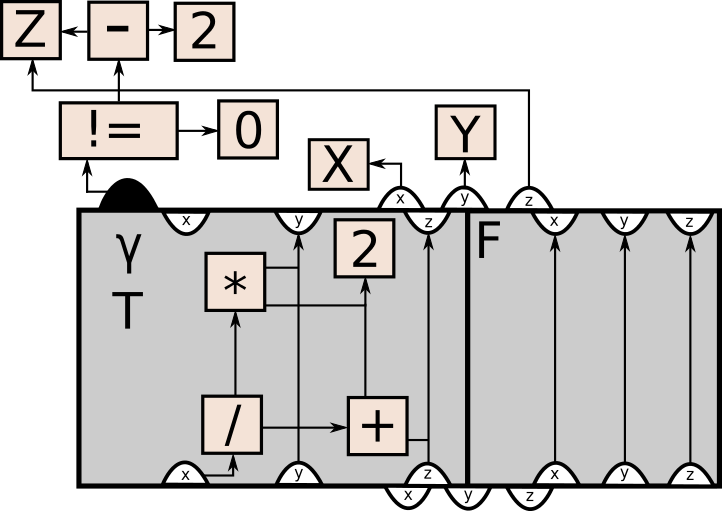
\includegraphics[width=\textwidth]{figures/simple_if_example}
	\end{minipage}
	\captionof{figure}{Example of an RVSDG subgraph equivalent to a simple C/C++ if-statement.}
	\label{fig:simple_if}
\end{centering}

\subsubsection{Edges}

The RVSDG has two types of edges: data dependence edges, and state dependence
edges, representing data and state dependencies one operation (node) has to
another, respectively. Data dependence edges are used to denote data
dependencies of an operation. An example of this being a variable used in an
addition. State dependence edges are used to preserve the semantics of the
program when the program has side-effecting operations, meaning that there are
no data dependencies between operations (nodes) that need to be performed in a
set order.

Figure~\ref{fig:simple_if} illustrates how data dependence edges work and look
like, and Figure~\ref{fig:factorial_loop_ex} shows how state dependence edges
are used and look like, in RVSDGs. We use dashed lines in this report to denote
state dependence edges in figures such as shown in
Figure~\ref{fig:factorial_loop_ex}.

\subsubsection{Nodes}

The RVSDG has two kinds of nodes: simple nodes and complex nodes. Simple nodes
are used in an RVSDG to represent simple operations, such as addition and
substraction. The arity and order of inputs and outputs of any RVSDG node need
to match across all the nodes representing the same operation.

However, simple nodes representing associative operations, such as
multiplication or equality-check, can switch the order of their inputs and still
yield the correct output. The same is not valid for non-associative operations,
such as division, substraction, and assignment operations.

The report puts special focus on the simple node called the \applyNode . An
\applyNode~represents the call site within an RVSDG of a function of the program
the RVSDG represents. The first argument of an \applyNode~is a link to the
complex node which represents the function the \applyNode~represents a call site
to. The rest of the input arguments of an \applyNode~need to match the order and
arity of the input arguments of the function-node it's linked to. Likewise, the
results also need to match the same order and arity as the outputs of the
function-node.

Complex nodes contain an RVSDG subgraph, which is why they are also referred to
as \textit{regions}. As simple nodes, complex nodes also need to have the same
order and arity of their inputs and outputs across all nodes representing an
equivalent operation.

Differing from the simple nodes with their contained subgraph, complex nodes
``gate'' the inputs they get from the rest of the RVSDG through to internal
outputs. Consequently, they also have internal inputs which gate through
to their external outputs, connecting the dependencies to the rest of the RVSDG.
The complex nodes of an RVSDG relevant for this report are as follows:

\begin{itemize}

\item \textbf{$\gamma$-nodes: N-way statements}

\textit{$\gamma$-nodes} represent conditional statements. Each $\gamma$-node has
a predicate as first input. All other edges passing as inputs to the
$\gamma$-node are edges its subregions depend upon. All subregions must have the
same order and arity of internal inputs and outputs, even if the subgraph in
each region does not depend on all of the internal outputs.

A $\gamma$-node is equivalent to a \textit{switch-case} without fall-through in
C/C++. Each case of the switch statement corresponds to a subregion of the
$\gamma$-node. Hence, a simple \textit{if-statement} with no else-clause can be
represented by a $\gamma$-node with two subregions. The true subregion contains
the RVSDG subgraph that represents the body of the if-statement, whereas the
false subregion of the $\gamma$-node simply routes all inputs through. See
Figure~\ref{fig:simple_if} for an example of a $\gamma$-node.

\item \textbf{$\theta$-nodes: Tail-controlled loops}

\textit{$\theta$-nodes} represent tail controlled loops. As with the
$\gamma$-node, its inputs (and outputs) are all the dependencies needed the
RVSDG subgraph in its subregion.

Inside the $\theta$-node there is an extra first internal input, which is
the predicate of the tail controlled loop. If this predicate evaluates to true,
the rest of the internal inputs of the $\theta$-node are mapped to their
corresponding internal outputs.

This enables the iterative behaviour of an RVSDG $\theta$-node. The new values
from the internal inputs of the previous iteration are mapped to the
internal outputs of the $\theta$-node. Then the operations represented by
its contained RVSDG subgraph are executed again with the new values.

A $\theta$-node is equivalent to a \textit{do-while} loop in C/C++, as shown in
Figure~\ref{fig:factorial_loop_ex}. See Listing~\ref{lst:factorial_loop_ex} for
the C/C++ code corresponding to the RVSDG depicted in
Figure~\ref{fig:factorial_loop_ex}.

\begin{lstlisting}[label={lst:factorial_loop_ex}, style=global_customcpp,
caption={C/C++ code corresponding to the RVSDG subgraph in
Figure~\ref{fig:factorial_loop_ex}.}]
int fac(unsigned int n){
	unsigned int i = 0;
	unsigned long long result = 1;
	do{
		i += 1;
		result *= i;
		std::cout << "Factorial #" << i << "\tis: " << result << std::endl;
		} while(i < n);
	}
	return result;
}
\end{lstlisting}
\vspace{-4\parskip} %http://tex.stackexchange.com/q/40863
\todo[inline]{Replace Figure~\ref{fig:factorial_loop_ex} with factorial
example!}

Other loops than tail-controlled loops can be represented by combining complex
nodes. A \textit{for-loop} can be represented by putting a $\theta$-node inside
of the \textit{true} clause of a $\gamma$-node conaining no subgraph in the
subregion representing the \textit{false} clause.

\begin{figure}[h!]
	\centering
	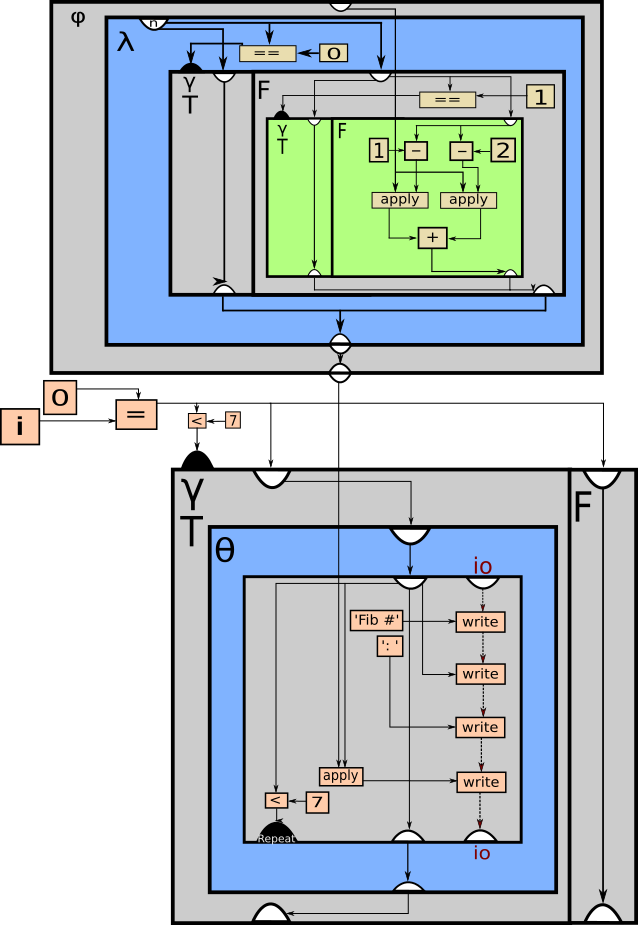
\includegraphics[width=\textwidth]{figures/for-loop-printf-rec_fib-example}
	\caption{An RVSDG representing the C/C++  program code in
Listing~\ref{lst:factorial_loop_ex}.}
	\label{fig:factorial_loop_ex}
\end{figure}

\clearpage
\item \textbf{$\lambda$-nodes: Functions}

A \textit{$\lambda$-node} contains an RVSDG subgraph representing operations
performed by a specific function. \textit{$\lambda$-nodes} only have internal
outputs and outputs, representing the arguments and results needed and given to
its contained RVSDG subgraph, respectively.

The invocation of a function represented by a \textit{$\lambda$-node} is
accomplished through linking the \textit{$\lambda$-node} to the \applyNode~at
the call site of the function in the RVSDG.

The external inputs of the \applyNode~are mapped to the internal outputs of the
\textit{$\lambda$-node}. This enables the evaluation of the body of the
\textit{$\lambda$-node}. The arity and order of its internal inputs and outputs
must match the arity and order of the external inputs and outputs of all
correspondingly linked \applyNode s. Thus the results of the
\textit{$\lambda$-node} are mapped to the results of the \applyNode .
Figure~\ref{fig:fib_phi} shows an RVSDG representation of a recursive fibonacci
function.

\item \textbf{$\phi$-regions: Recursive environments}

\textit{$\phi$-regions} contain at least one recursive \textit{$\lambda$-node}.
Like the \textit{$\lambda$-node}, it only has internal inputs and outputs. The
internal outputs of the \textit{$\phi$-region} connect to the links used by the
\applyNode s within it to link to their respective \textit{$\lambda$-nodes}, if
these are also present within the same \textit{$\phi$-region}. The internal
inputs of a \textit{$\phi$-region} link to the \textit{$\lambda$-nodes}
contained within. Thus enabling \applyNode s outside of the recursive
environment to link with the \textit{$\lambda$-nodes} contained within.

An RVSDG representing a recursive fibonacci function illustrates the usage of
a \textit{$\phi$-region} in Figure~\ref{fig:fib_phi}.

\end{itemize}

\begin{lstlisting}[label={lst:fib_phi}, style=global_customcpp,
caption={C/C++ code corresponding to the RVSDG subgraph in
Figure~\ref{fig:fib_phi}.}]
int fib(unsigned int n){
	if (n < 2){
		return n;
	}
	return fib(n-1) + fib(n-2);
}
\end{lstlisting}
\vspace{-4\parskip} %http://tex.stackexchange.com/q/40863

\begin{figure}[h!]
	\centering
	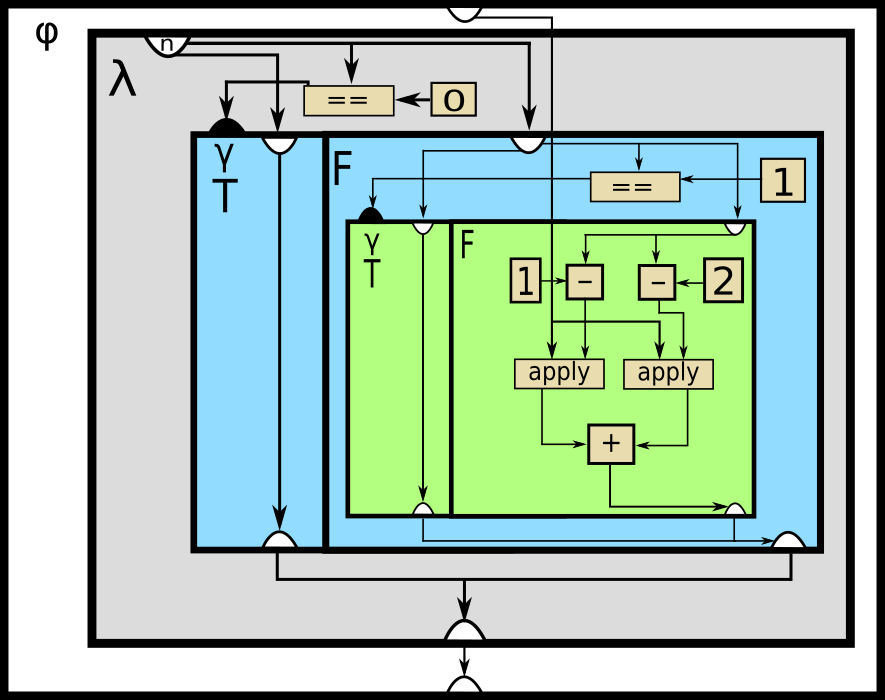
\includegraphics[width=\textwidth]{figures/recursive_fibonacci}
	\caption{A $\phi$-node containing a $\lambda$-node representing a recursive
version of a function producing the \lstinline!n! first numbers in the Fibonacci
series.}
	\label{fig:fib_phi}
\end{figure}
